% Created 2019-12-12 Thu 15:29
% Intended LaTeX compiler: pdflatex
\documentclass[aspectratio=169]{beamer}
\usepackage[utf8]{inputenc}
\usepackage[T1]{fontenc}
\usepackage{graphicx}
\usepackage{grffile}
\usepackage{longtable}
\usepackage{wrapfig}
\usepackage{rotating}
\usepackage[normalem]{ulem}
\usepackage{amsmath}
\usepackage{textcomp}
\usepackage{amssymb}
\usepackage{capt-of}
\usepackage{hyperref}
\usetheme{UoB}
\author{Mark Blyth}
\date{2019-12-16 Mon}
\title{Electrophysiology methods for neural bifurcation analysis}
\hypersetup{
 pdfauthor={Mark Blyth},
 pdftitle={Electrophysiology methods for neural bifurcation analysis},
 pdfkeywords={},
 pdfsubject={},
 pdfcreator={Emacs 26.3 (Org mode 9.1.9)}, 
 pdflang={English}}
\begin{document}

\maketitle

\section{Intro to my project}
\label{sec:org4e2005f}
\begin{frame}[label={sec:org6dac2e5}]{Presentation plan}
\begin{itemize}
\item \alert{30 second overview of my project}
\item Overview of my mircrofluidics questions
\item Review of potential solutions
\end{itemize}
\end{frame}
\begin{frame}[label={sec:org734db4a}]{About my project}
\begin{itemize}
\item Hodgin and Huxley provided a model of neural dynamics
\item It turns out we can explain all observations from classical neuroscience using dynamical systems theory
\item These explanations typically focus on the bifurcations a neuron can exhibit
\item Bifurcations are analysed from models; I'm wanting to do a bifurcation analysis on a real, living neuron
\item Goal: consider a single neuron, and experimentally find  bifurcations in its dynamics
\end{itemize}

\end{frame}
\begin{frame}[plain]

\begin{center}
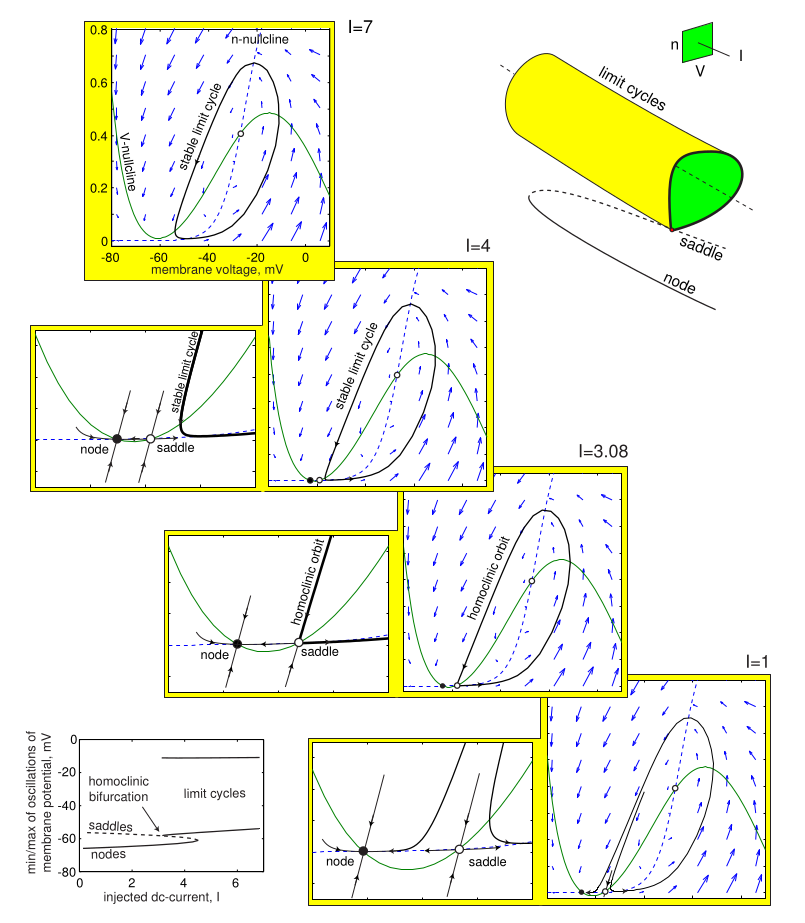
\includegraphics[height=1.4\textheight]{./homoclinic.png}
\end{center}
\end{frame}

\begin{frame}[label={sec:org9b4670d}]{Presentation plan}
\begin{itemize}
\item 30 second overview of my project
\item \alert{Overview of my mircrofluidics questions}
\item Review of potential solutions
\end{itemize}
\end{frame}
\begin{frame}[label={sec:orgdac3cf6}]{The big question}
The dynamics of any given neuron typically change when current is injected into that neuron. I'm wanting to observe and control these changes experimentally.
I need an experimental setup that would allow me to\ldots{}
\begin{itemize}[<+->]
\item Apply a current into a neuron
\item Observe that neuron's membrane potential
\item Keep the neuron alive as long as possible
\item (If it were possible, also measure each ion channel's average conductance)
\end{itemize}

QUESTION: what would be an appropriate experimental setup to achieve this?
\end{frame}


\section{Methods}
\label{sec:org52f1efc}
% Mention here that I'm going to talk through the different methods I've researched, with the goal being to pick one of them to develop further for the next THETA project
\begin{frame}[label={sec:org0c27409}]{Presentation plan}
\begin{itemize}
\item 30 second overview of my project
\item Overview of my mircrofluidics questions
\item \alert{Review of potential solutions}
\end{itemize}
\end{frame}
\begin{frame}[label={sec:orga50b009}]{Bath MEA}
\begin{itemize}
\item Idea:
\begin{itemize}
\item Use the current microfluidics device, or a minor modification of it
\end{itemize}
\item Strengths:
\begin{itemize}
\item Builds on existing work and expertise
\end{itemize}
\item Weaknesses:
\begin{itemize}
\item Can't isolate the dynamics of an individual neuron
\item Can't give a specific neuron a current input
\item Can't measure membrane potentials
\end{itemize}
\end{itemize}
% Why do I think it's inappropriate for my project?
% How much would I need to change in order to use it?
\end{frame}

\begin{frame}[label={sec:org2d93f96}]{Glass pipette patch clamp}
\begin{itemize}
\item Idea:
\begin{itemize}
\item Use the classical glass pipette method for a whole-cell patch clamp
\item Measure membrane potential and inject current using the electrode
\end{itemize}
\item Strengths:
\begin{itemize}
\item Allows for studying the dynamics of individual neurons
\item Easy to inject current, and to measure membrane potential
\end{itemize}
\item Weaknesses:
\begin{itemize}
\item Patch clamping can be difficult
\item Neuron might not survive as long since we can't control nutrients and waste as easily
\end{itemize}
\end{itemize}
% Explain why patch clamping is more useful for me
% Discuss its limitations (cells die faster, can't control exterior environment easily, hard to do)
\end{frame}

\begin{frame}[label={sec:orgec9fe43}]{Off-the-shelf automated patch clamp}
\begin{itemize}
\item Idea:
\begin{itemize}
\item Same as before, but use an automated machine to do the patch clamping
\end{itemize}
\item Strengths:
\begin{itemize}
\item Allows for studying the dynamics of individual neurons
\item Easy to inject current, and to measure membrane potential
\item Much easier than manual patch clamping, no training required
\item Allows constant perfusion for providing nutrients and removing waste
\end{itemize}
\item Weaknesses:
\begin{itemize}
\item More expensive than DIY methods (unless we can borrow a machine from somewhere)
\item Might be hard to interface with a custom CBC control system
\end{itemize}
\end{itemize}
\end{frame}

\begin{frame}[label={sec:org30fb1c7}]{DIY microfluidic patch clamper}
\begin{itemize}
\item Idea:
\begin{itemize}
\item Combine the MEA and patch clamping methods
\item Build a planar patch clamping microfluidics device in-house
\end{itemize}
\item Strengths:
\begin{itemize}
\item Allows for studying the dynamics of individual neurons
\item Easy to inject current, and to measure membrane potential
\item Much easier than manual patch clamping, no training required
\item Allows constant perfusion for providing nutrients and removing waste
\item Cheaper and more customisable than buying a machine
\end{itemize}
\item Weaknesses:
\begin{itemize}
\item Need to design another microfluidics device
\end{itemize}
\end{itemize}

\end{frame}
\begin{frame}[plain]

\begin{center}
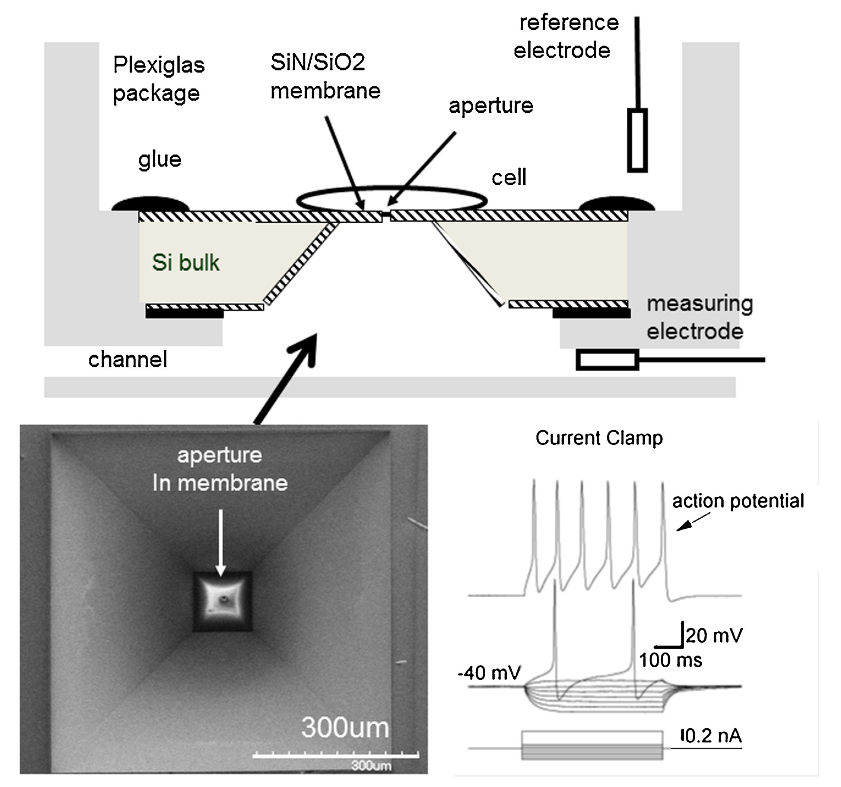
\includegraphics[height=1.4\textheight]{./planarpatch1.png}
\end{center}
\end{frame}

\begin{frame}[label={sec:orgd394775}]{Microfluidics fluorescence chip}
\begin{itemize}
\item Idea:
\begin{itemize}
\item Use an existing microfluidics chip, built for GFP imaging
\item Use calcium imaging to observe a neuron's behaviour
\end{itemize}

\item Strengths:
\begin{itemize}
\item Recently developed proteins allow the observations of individual action potentials
\item Might be able to estimate membrane potential from calcium imaging
\item Would allow the use of off-the-shelf chips, with no further developments
\end{itemize}

\item Weaknesses:
\begin{itemize}
\item No obvious way to inject current into the neuron, so any control inputs would have to be pharmacological
\item Probably can't investigate the dynamics of single isolated cells, only networks
\end{itemize}
\end{itemize}
% BRIEF ASIDE
% Could use calcium imaging to measure neural activity
% This lacks any way to stimulate the neuron, so if I want to inject current I'd end up turning it into one of the other devices instead
% (but, could use this and inject drugs to alter ion channel activity)
% [[https://scholar.google.com/scholar?hl=en&as_sdt=0%2C5&q=Nature%2C+499%3A295%E2%80%93300%2C+2013&btnG=][Paper introducing high-sensitivity calcium imaging]]
\end{frame}


\section{Reprise}
\label{sec:orgfa0337e}
\begin{frame}[label={sec:org43dcf2c}]{The big question (again)}
Which of these methods would best allow me to\ldots{}
\begin{itemize}
\item Apply a current into a neuron
\item Observe that neuron's membrane potential
\item Keep the neuron alive as long as possible
\item (If it were possible, also measure each ion channel's average conductance)
\end{itemize}
\end{frame}
\end{document}
